\documentclass{zjusct-beamer/zjusctbeamer}

% Metadata
\title{Introduction to Computer Systems in HPC}
\subtitle{Day 1 - The Hidden World Beneath Your Code}
\author[YooLc]{Chenxiao Li (@YooLc)}
\date{\today}
\institute[ZJUSCT]{Zhejiang University Supercomputing Team}
\copyleftnotice{CC-BY 4.0}

\hypersetup{
    pdftitle={\title},
    pdfpagemode=FullScreen,
}

\begin{document}

% Set Mono and Emoji font
\setmonofont{DejaVu Sans Mono}
\setemojifont{TwemojiMozilla}

\maketitle

% Outline (Table of Contents)
\cutoc

% Slide 正文均使用英文
\section{Introduction}

% 我的简介
\begin{frame}[fragile]{\emoji{bust-in-silhouette} Biography}
	\begin{center}
		\begin{itemize}
			\item \textbf{Baolin Zhu} (\emoji{bowling} @bowling233)
			\item (with Eric) Leader of ZJUSCT
			\item \textbf{Research Interests}: Arch/OS, Three Pillars (Compute, Network and Storage)
		\end{itemize}
		\begin{tikzpicture}
			% Timeline base line
			\draw[thick, gray] (0,0) -- (10.5,0);

			% Node 0: CKC AGC
			\fill[blue] (1.5, 0) circle (0.1);
			\draw[gray] (1.5, 0) -- (1.5, 0.5);
			\node at (1.5, 1) {
\includegraphics[width=0.8cm]{day8_pm/img/bio-ckcagc.png}};
			\node[font=\bfseries\small] at (1.5, 2) {CKC AGC};
			\node[font=\footnotesize, gray] at (1.5, -0.5) {Freshman};

			% Node 1: ZJUSCT
			\fill[blue] (4.0, 0) circle (0.1);
			\draw[gray] (4.0, 0) -- (4, 0.5);
			\node at (4.0, 1) {
\includegraphics[width=0.8cm]{day8_pm/img/bio-zjusct.png}};
			\node[font=\bfseries\small] at (4.0, 2) {ZJUSCT};
			\node[font=\footnotesize, gray] at (4.0, -0.5) {Sophomore};

			% Node 2: RC4ML Lab
			\fill[blue] (6.5, 0) circle (0.1);
			\draw[gray] (6.5, 0) -- (6.5, 0.5);
			\node at (6.5, 1) {
\includegraphics[width=0.8cm]{day8_pm/img/bio-rc4ml.png}};
			\node[font=\bfseries\small] at (6.5, 2) {RC4ML Lab};
			\node[font=\footnotesize, gray] at (6.5, -0.5) {Junior};

			% Node 3: Tencent
			\fill[blue] (9.0, 0) circle (0.1);
			\draw[gray] (9.0, 0) -- (9.0, 0.5);
			\node at (9.0, 1) {
\includegraphics[width=0.8cm]{day8_pm/img/bio-csig.png}};
			\node[font=\bfseries\small] at (9.0, 2) {Tencent CSIG};
			\node[font=\footnotesize, gray] at (9.0, -0.5) {Junior};

		\end{tikzpicture}
	\end{center}
\end{frame}

% 本节课的参考教材
\begin{frame}[fragile]{\emoji{books} Textbook}

	\begin{columns}
		\begin{column}{0.4\textwidth}
			\begin{center}
				
\includegraphics[width=0.8\textwidth]{day8_pm/img/1-book.png}
			\end{center}

		\end{column}
		\begin{column}{0.6\textwidth}
			\begin{itemize}
				\item \textbf{Title}: C++ Concurrency in Action (Second Edition)
				\item \textbf{Authors}: Anthony Williams
				\item \textbf{Publisher}: Manning Publications
			\end{itemize}
		\end{column}
	\end{columns}
\end{frame}

% 本节课的内容大纲
\begin{frame}[fragile]{\emoji{book} Outline}
\section{Operating System Basics}
\subsection{Introduction}

\begin{frame}[fragile]{Abstraction of CPU}

	Take a closer look at the CPU die:

	\only<1>{
		\begin{figure}[H]
			\centering
			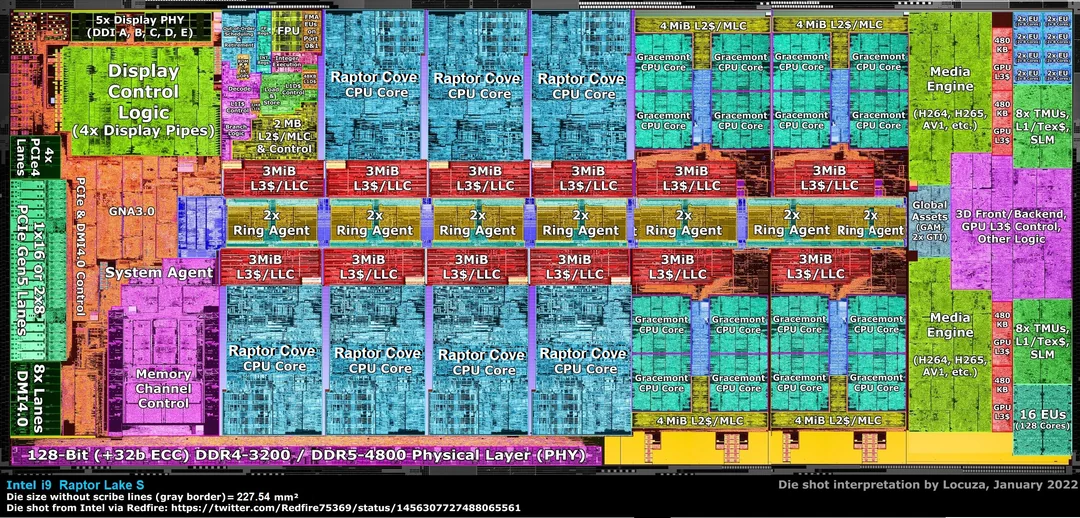
\includegraphics[width=0.75\textwidth]{day3/img/cpu-die.png}
			\caption{Intel Core i9 13900K Die Shot}
		\end{figure}
	}

	\only<2->{
		\begin{columns}
			\begin{column}{0.6\textwidth}
				\begin{figure}[H]
					\centering
					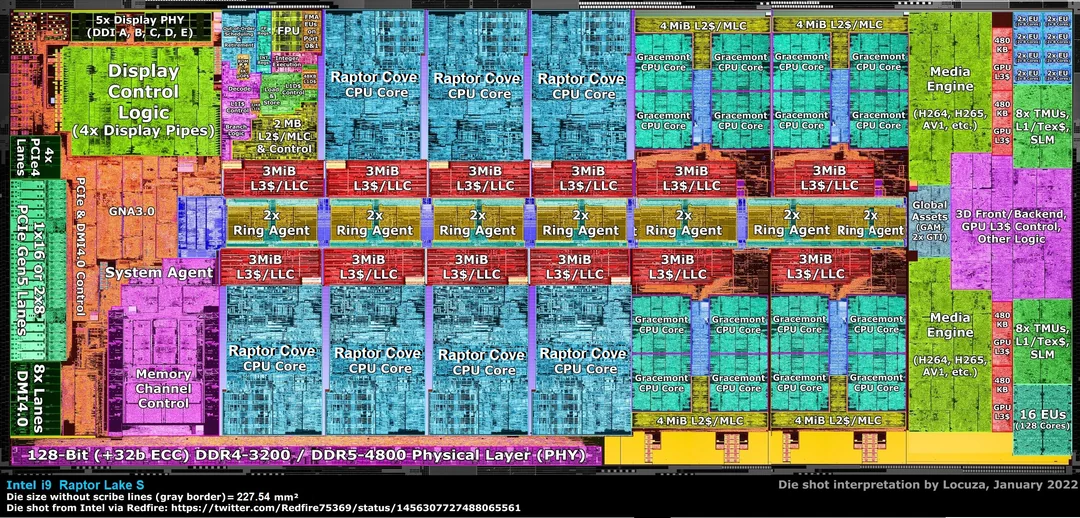
\includegraphics[width=\textwidth]{day3/img/cpu-die.png}
				\end{figure}
			\end{column}
			\begin{column}{0.4\textwidth}
				\begin{figure}[H]
					\centering
					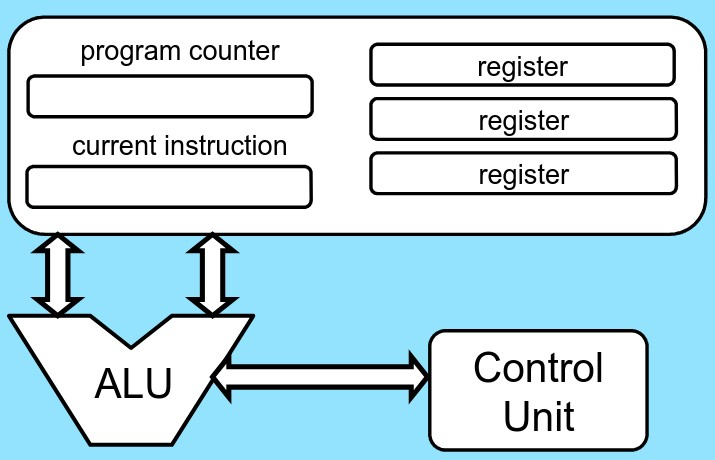
\includegraphics[width=\textwidth]{day3/img/cpu-abstract.jpg}
				\end{figure}
			\end{column}
		\end{columns}

		\begin{itemize}
			\item<3-> \textbf{Program Counter}
			\item<4> Register: stores data processed by the CPU (\textbf{a.k.a. context})
		\end{itemize}

	}

\end{frame}

\begin{frame}[fragile]{Memory Hierarchy}
	\only<1>{
		\begin{figure}[H]
			\centering
			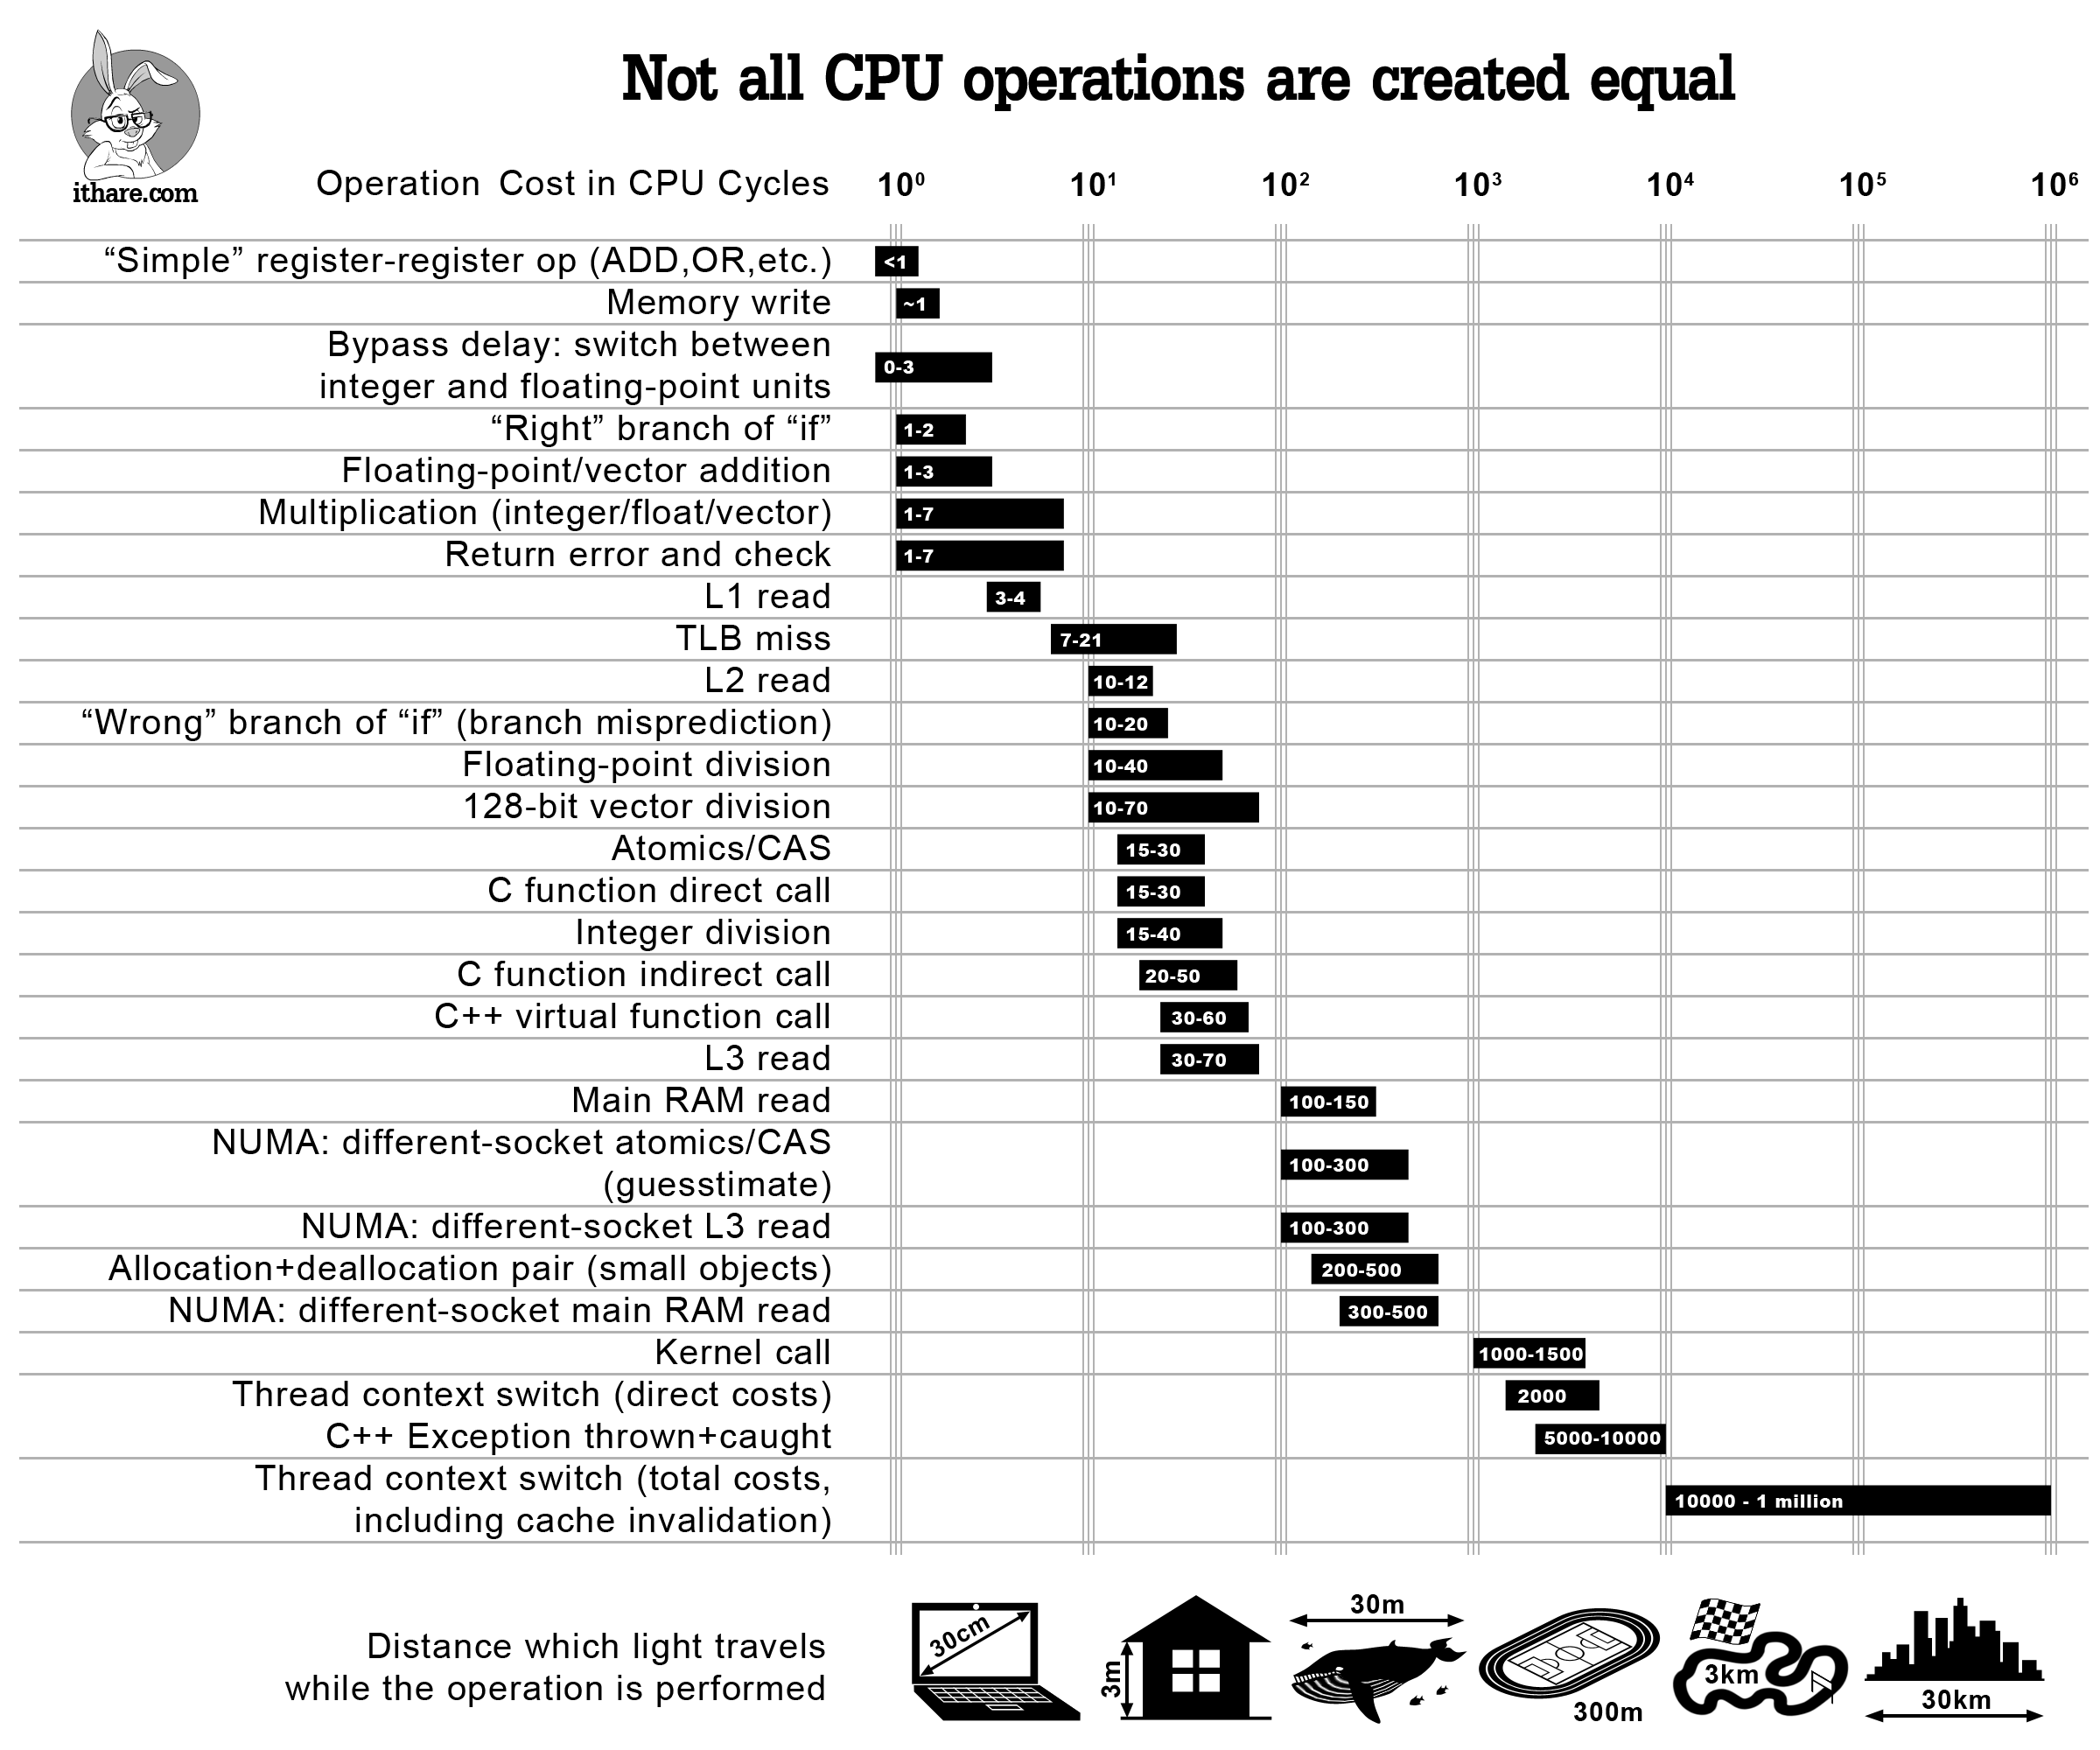
\includegraphics[width=0.55\textwidth]{day3/img/latency-2.png}
		\end{figure}
	}
	\only<2>{
		\begin{figure}[H]
			\centering
			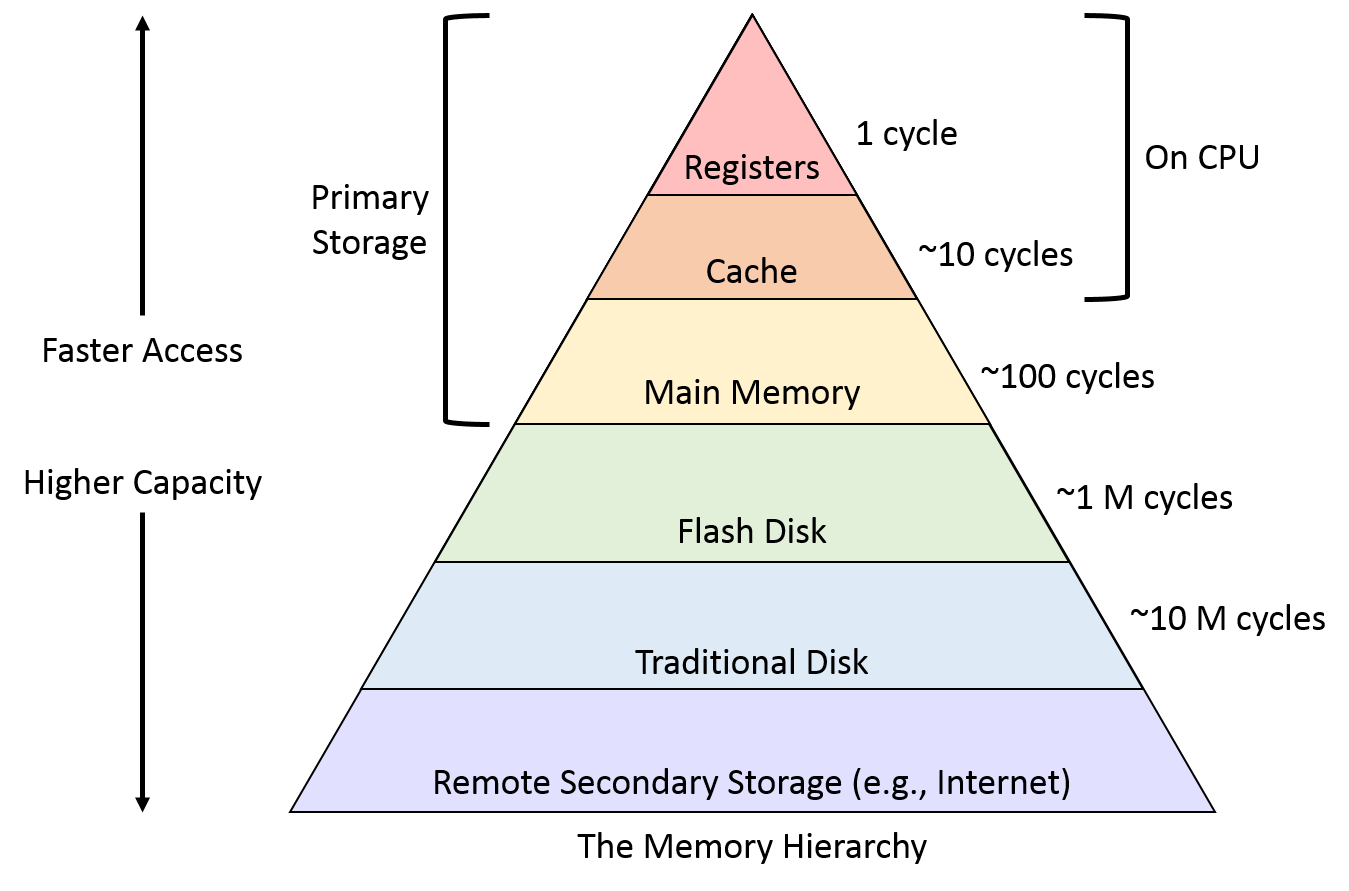
\includegraphics[width=0.7\textwidth]{day3/img/mem-hi.png}
		\end{figure}
	}
\end{frame}

\begin{frame}[fragile]{\emoji{thinking} What is an Operating System?}
	Common operating systems we see in 2025:
	\begin{columns}[T]
		\begin{column}{0.6\textwidth}
			\begin{figure}[H]
				\centering
				
\includegraphics[width=0.8\textwidth]{day3/img/123.png}
			\end{figure}
		\end{column}
		\begin{column}{0.4\textwidth}
			\begin{minipage}[c][.5\textheight][c]{\linewidth}
				\begin{itemize}
					\item Windows\onslide<2>{:\textbf{ NT}}
					\item macOS, iOS\onslide<2>{:\textbf{ Darwin}}
					\item Linux, Android\onslide<2>{:\textbf{ Linux}}
				\end{itemize}
			\end{minipage}
		\end{column}
	\end{columns}
	\onslide<3>{
		\emoji{star} Operating System is \textbf{resource abstractor and resource allocator}.
	}
\end{frame}

\begin{frame}[fragile]{10k meter view of kernel code}
	\begin{columns}[T]
		\begin{column}{0.75\textwidth}
			\begin{minted}[fontsize=\small]{c}
void processEvent(event) {
    switch (event.type) {
        case NETWORK_COMMUNICATION:
            NetworkManager.handleEvent(event);
            break;
        case SEGMENTATION_FAULT:
        case INVALID_MODE:
            ProcessManager.handleEvent(event);
            break;
        // ...
    }
}
        \end{minted}
		\end{column}
		\begin{column}{0.2\textwidth}
			\begin{minipage}[c][.6\textheight][c]{\linewidth}
				\begin{itemize}
					\item \textbf{Event}
					\item \textbf{Handler}
				\end{itemize}
			\end{minipage}
		\end{column}
	\end{columns}
\end{frame}

\subsection{OS Events}


\begin{frame}[fragile]{OS Events}

	There are two kinds of events, we call them \textbf{Traps} in RISC-V\footnotemark:

	\begin{itemize}
		\item \textbf{Interrupts}: external asynchronous events
		      \begin{itemize}
			      \item Hardware-generated
			      \item e.g., some device controller says “something happened”
		      \end{itemize}
		\item \textbf{Exceptions}: unusual condition occurring at instruction run time
		      \begin{itemize}
			      \item Software-generated
			      \item e.g. a division by zero
		      \end{itemize}
	\end{itemize}

	\footnotetext{\href{https://zju-arch.pages.zjusct.io/arch-sp25/spec/riscv-unprivileged.html\#trap-defn}{1.6. Exceptions, Traps, and Interrupts}, RISC-V Unprivileged ISA Specification}

\end{frame}

\begin{frame}[fragile]{Trapped Control Flow}
	When a trap occurs, the control flow is switched to its handler:
	\begin{columns}
		\begin{column}{0.6\textwidth}
			\begin{figure}[H]
				\centering
				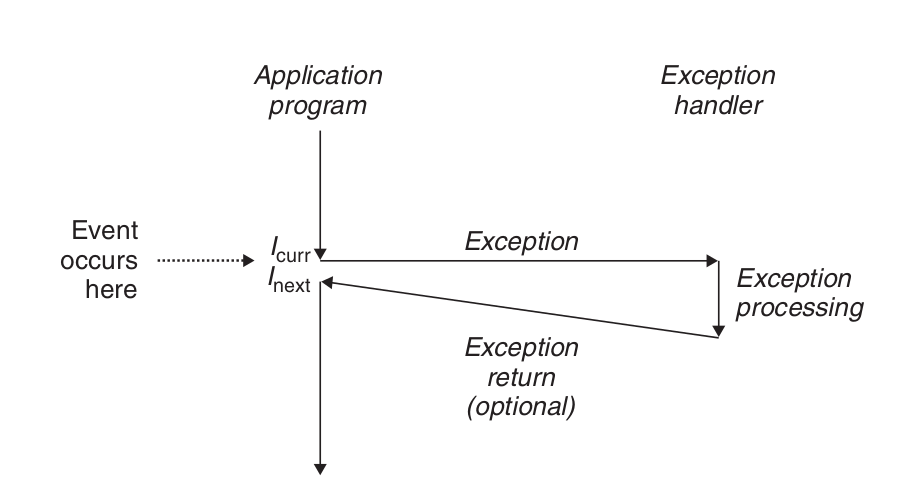
\includegraphics[width=\textwidth]{day3/img/interrupt-flow.png}
			\end{figure}
		\end{column}
		\begin{column}{0.4\textwidth}
			\only<1-2>{
				\begin{figure}[H]
					\centering
					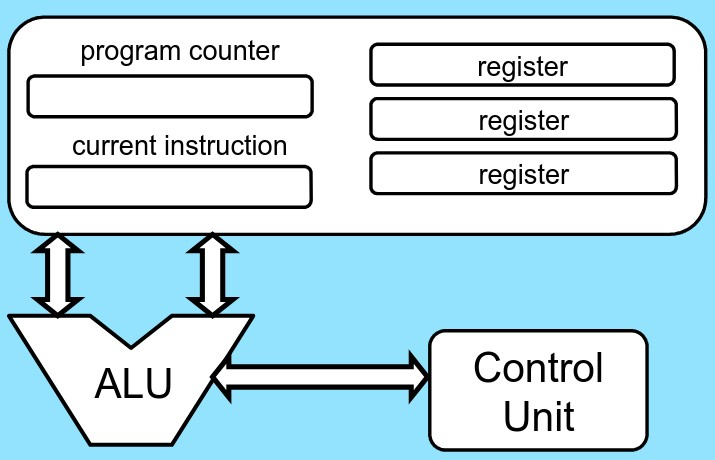
\includegraphics[width=\textwidth]{day3/img/cpu-abstract.jpg}
				\end{figure}
			}
			\only<3>{
				\begin{figure}[H]
					\centering
					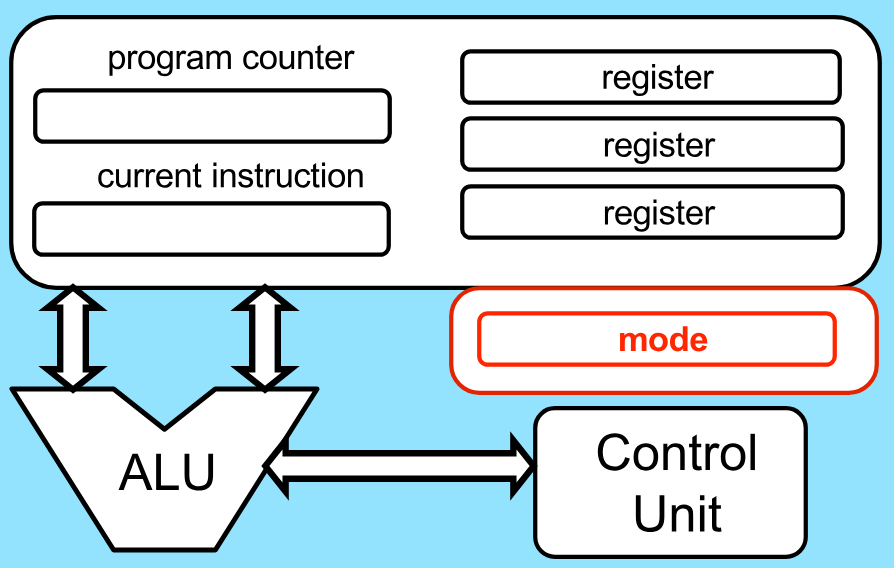
\includegraphics[width=\textwidth]{day3/img/mode-bit.png}
				\end{figure}
			}
		\end{column}
	\end{columns}
	\onslide<2->{\emoji{thinking} \textbf{Q: What do we need to separate the user and kernel space?}}

	\onslide<3>{\emoji{smirk} A: Add a \textbf{Mode Bit} to keep track of the current \textbf{privilege level}.}
\end{frame}


% \section{System Call}

\begin{frame}[fragile]{System Calls}
	When a user program needs to do something privileged, it \textbf{calls a system call}. A system call is a special kind of trap.
	\begin{figure}[H]
		\centering
		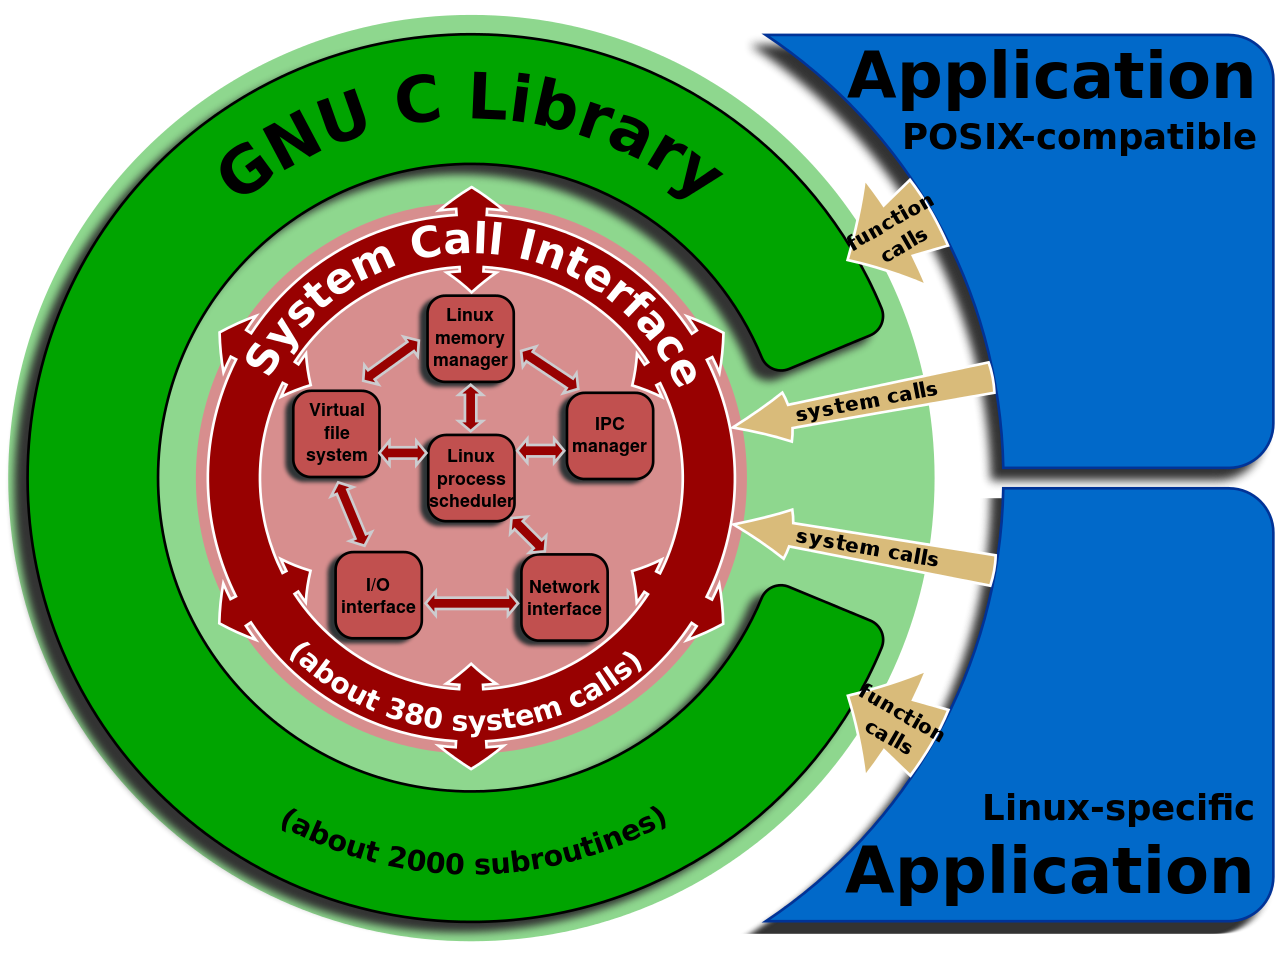
\includegraphics[width=0.5\textwidth]{day3/img/syscall.png}
	\end{figure}

\end{frame}

\begin{frame}[fragile]{10k meter view of kernel code (revised)}
	\begin{minted}[fontsize=\scriptsize,highlightlines={10-12}]{c}
void processEvent(event) {
    switch (event.type) {
        case NETWORK_COMMUNICATION:
            NetworkManager.handleEvent(event);
            break;
        case SEGMENTATION_FAULT:
        case INVALID_MODE:
            ProcessManager.handleEvent(event);
            break;
        case SYSTEM_CALL:
            SystemCallManager.handleEvent(event);
            break;
        // ...
    }
}
    \end{minted}
\end{frame}

\begin{frame}[fragile]{System Call Handler}
	\begin{figure}[H]
		\centering
		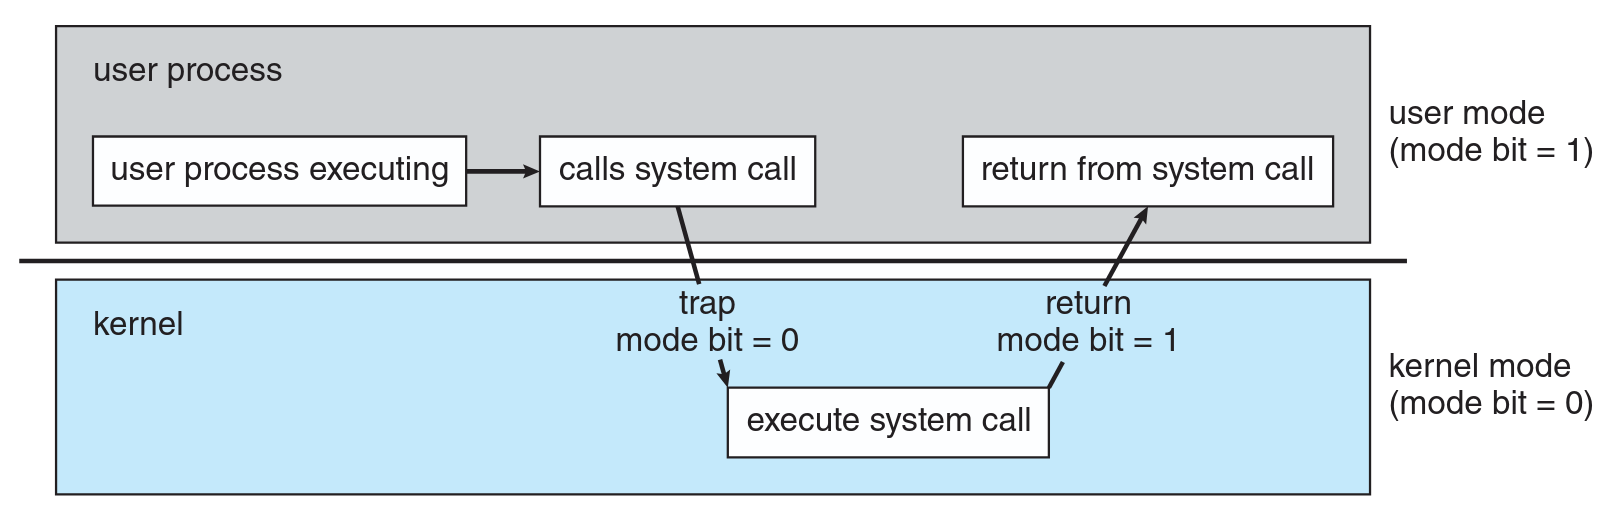
\includegraphics[width=\textwidth]{day3/img/interrupt.png}
	\end{figure}
\end{frame}

\begin{frame}[fragile]{Timers}
	\begin{itemize}
		\item The OS must keep control of the CPU
		      \begin{itemize}
			      \item Programs cannot get stuck in infinite loop and lock up the computer
			      \item Programs cannot gain an unfair share of the computer
		      \end{itemize}
		\item One way in which the kernel retrieves
		      control is when an interrupt occurs
		\item To make sure that an interrupt will occur reasonably soon, we can use a timer
	\end{itemize}
\end{frame}

\begin{frame}[fragile]{10k meter view of kernel code (revised)}
	\begin{minted}[fontsize=\scriptsize,highlightlines={3-5}]{c}
void processEvent(event) {
    switch (event.type) {
        case TIMER_INTERRUPT:
            TimerManager.handleEvent(event);
            break;
        // ...
        case SYSTEM_CALL:
            SystemCallManager.handleEvent(event);
            break;
        // ...
    }
}
    \end{minted}
\end{frame}

\section{Process}

\begin{frame}[fragile]{\emoji{thinking} What's inside a program?}

	\emoji{star} A process is \textbf{a program in execution, a unit of resource allocation and protection.}

	Let's see what makes up a program:
	\begin{minted}[fontsize=\scriptsize]{bash}
$ gcc hello.c -o hello
$ ./hello
Hello World!
$ file hello
hello: ELF 64-bit LSB pie executable, x86-64, version 1 (SYSV),
 dynamically linked, interpreter /lib64/ld-linux-x86-64.so.2,
 BuildID[sha1]=c6fe8ac2e5be3c78cf31179a5cb31df3978ca160,
 for GNU/Linux 3.2.0, not stripped
\end{minted}
\end{frame}

\begin{frame}[fragile]{ELF: Executable and Linkable Format}
	\only<1>{
		% \begin{columns}
		%     \begin{column}{0.8\textwidth}
		\begin{figure}[H]
			\centering
			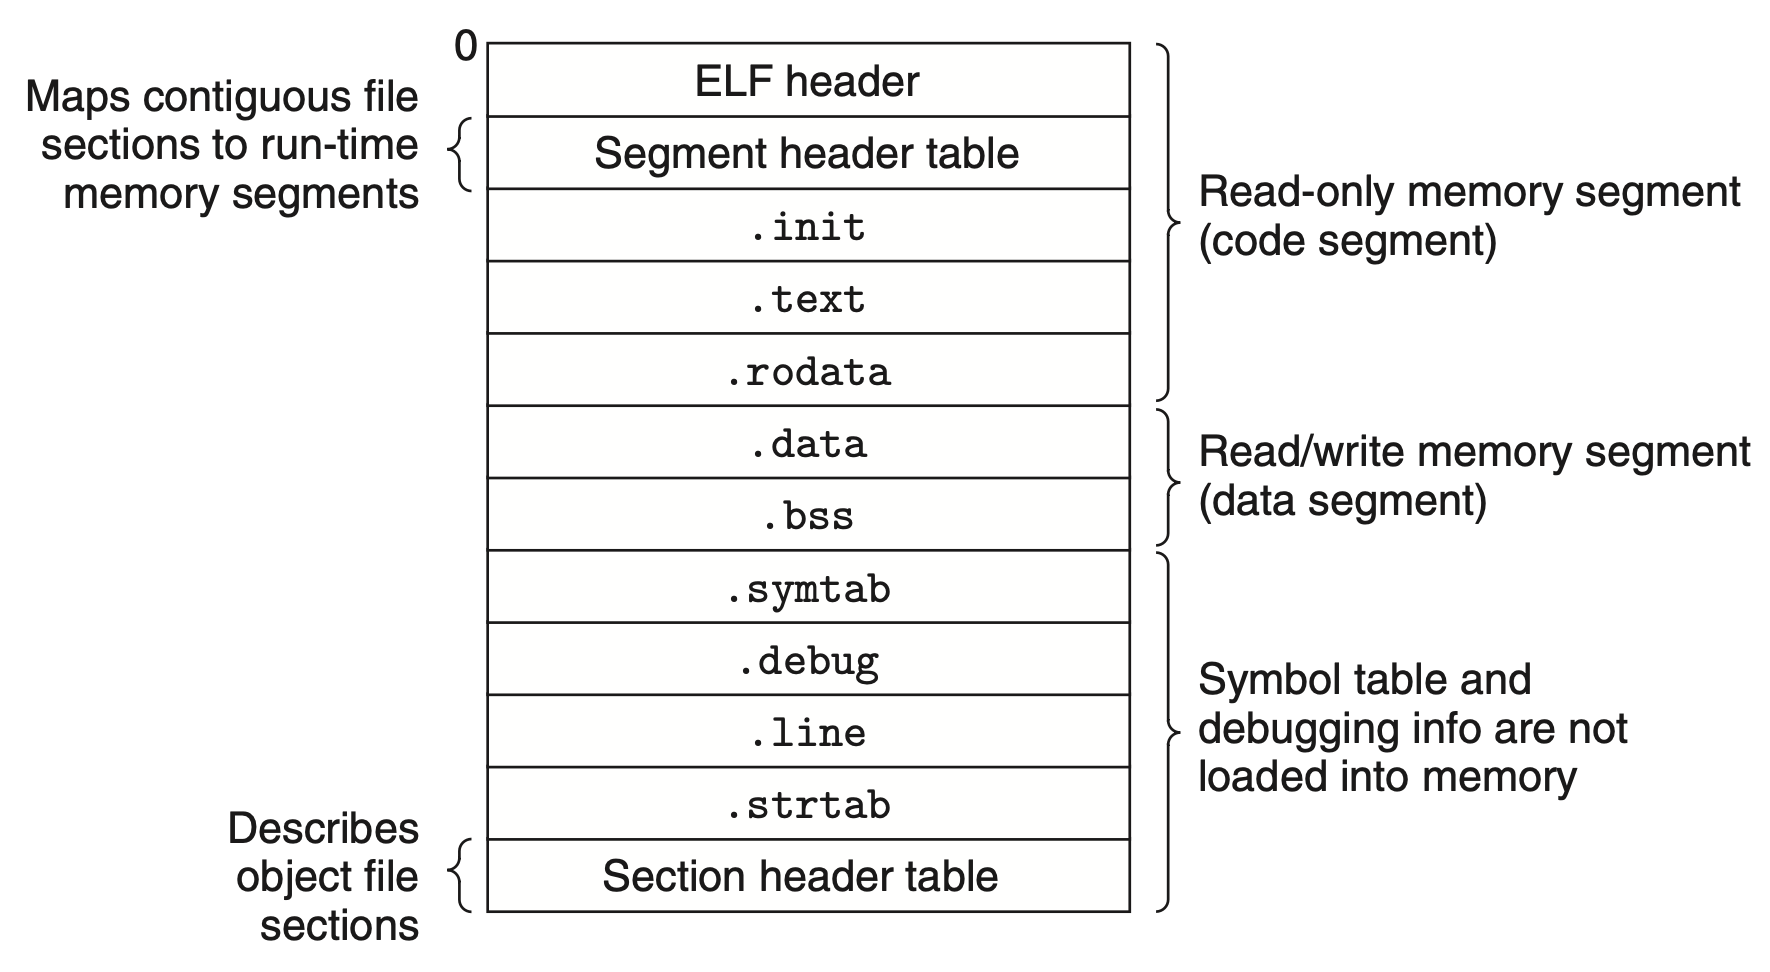
\includegraphics[width=0.75\textwidth]{day3/img/elf-layout-2.png}
			\caption{ELFs are organized into sections}
		\end{figure}
		%     \end{column}
		%     \begin{column}{0.2\textwidth}
		%         123
		%     \end{column}
		% \end{columns}
	}

	% \only<2>{
	%     \begin{tabular}{c|c|c}
	%         \hline
	%         \textbf{Section} & \textbf{W} & \textbf{X}\\
	%         \hline
	%         \verb|.text| & No & Yes \\
	%         \verb|.rodata| & No & No \\
	%         \verb|.data| & Yes & No \\
	%         \verb|.bss| & Yes & No \\
	%         \hline
	%     \end{tabular}
	% }
\end{frame}

\begin{frame}[fragile]{Process Address Space}
	\begin{columns}
		\begin{column}{0.3\textwidth}
			\begin{figure}[H]
				\centering
				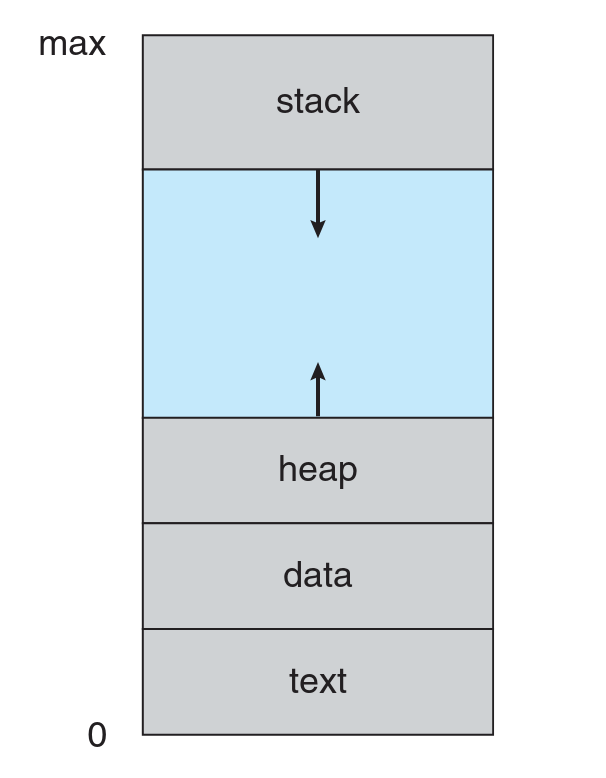
\includegraphics[width=\textwidth]{day3/img/process-layout.png}
			\end{figure}
		\end{column}
		\begin{column}{0.7\textwidth}
			A Process = A Program in Execution =
			\begin{itemize}
				\item<1-> \textbf{In Memory (Unique Address Space)}:
				      \begin{itemize}
					      \item \textbf{Code}: Text section, initially stored on disk
					      \item<2-> \textbf{Data Section}:
					            \begin{itemize}
						            \item \textbf{BSS}: Uninitialized data
						            \item \textbf{Data}: Initialized data
					            \end{itemize}
					      \item<3-> \textbf{Stack}: Function frames, local variables, etc.
					      \item<3-> \textbf{Heap}: Dynamic memory allocation
				      \end{itemize}
				\item<4-> \textbf{Context}:
				      \begin{itemize}
					      \item \textbf{Program Counter}: Points to the next instruction to execute (i.e., an address in the code)
					      \item Content of the processor's \textbf{registers}
				      \end{itemize}
			\end{itemize}
		\end{column}
	\end{columns}
\end{frame}

% \begin{frame}[fragile]{ELF Cheatsheet}
%     \begin{figure}[H]
%         \centering
%         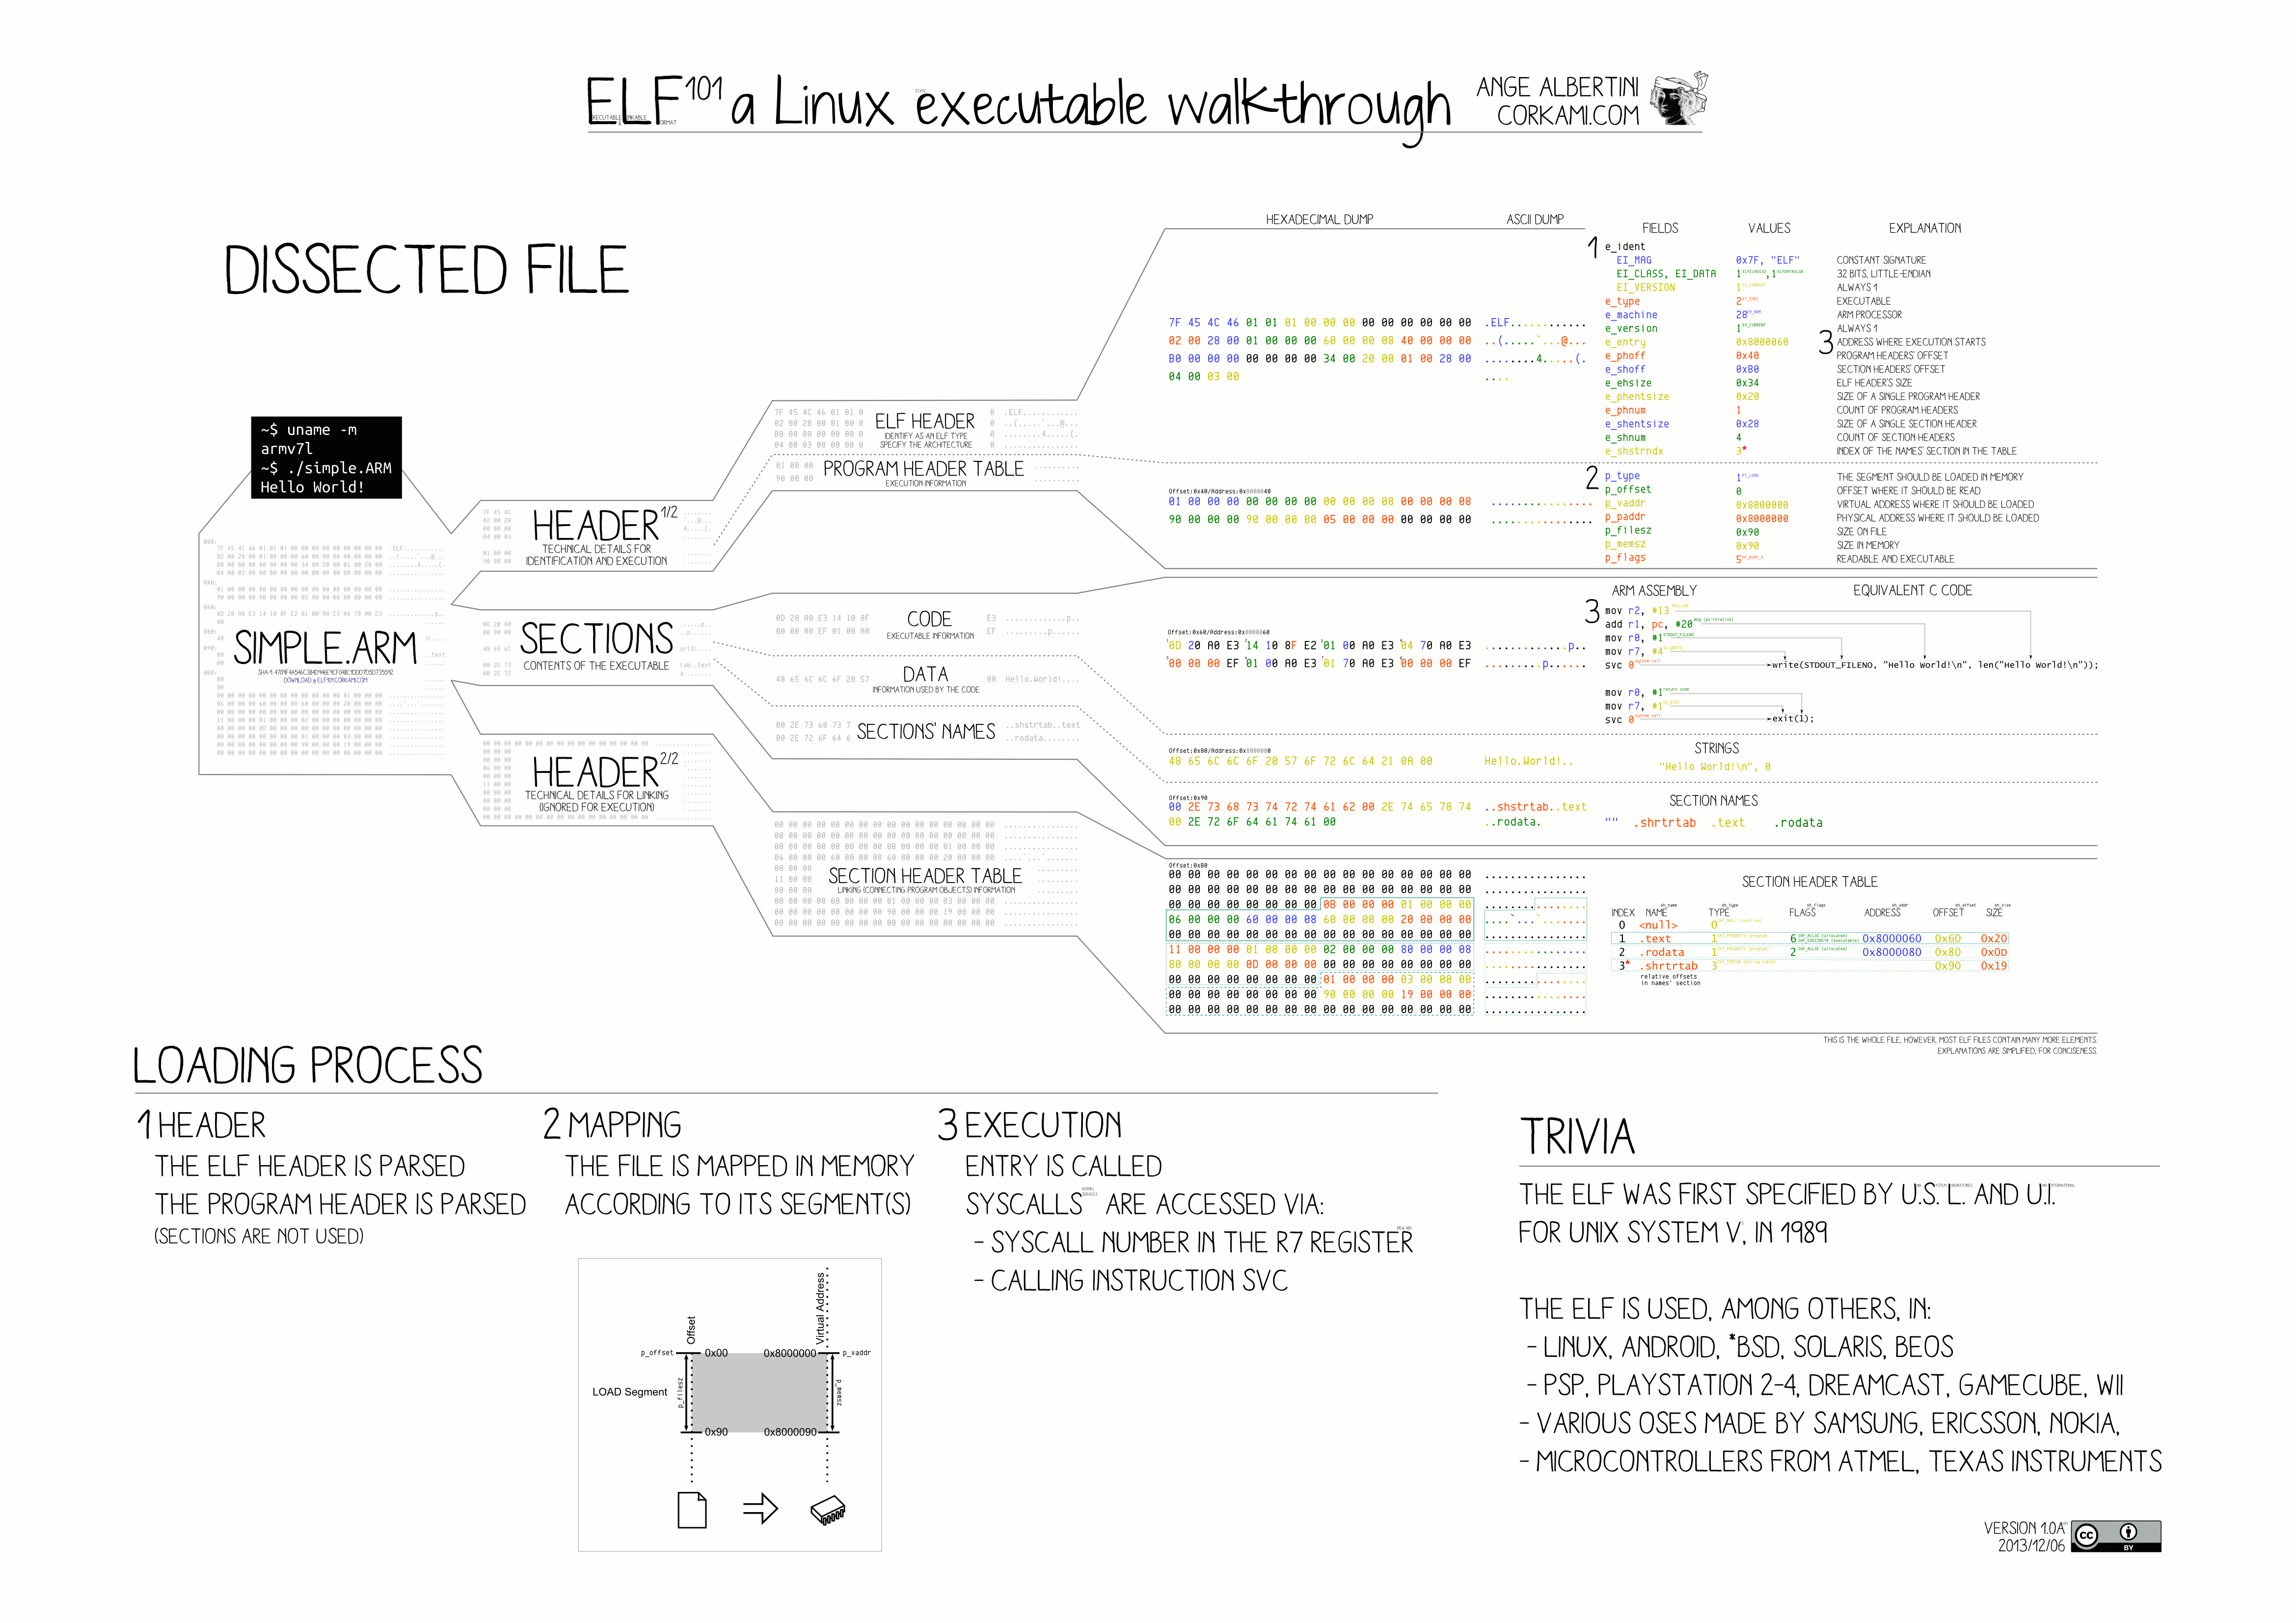
\includegraphics[width=\textwidth]{day3/img/elf-cheatsheet.png}
%     \end{figure}
% \end{frame}

\begin{frame}[fragile]{Stack Frame}
	\begin{figure}[H]
		\centering
		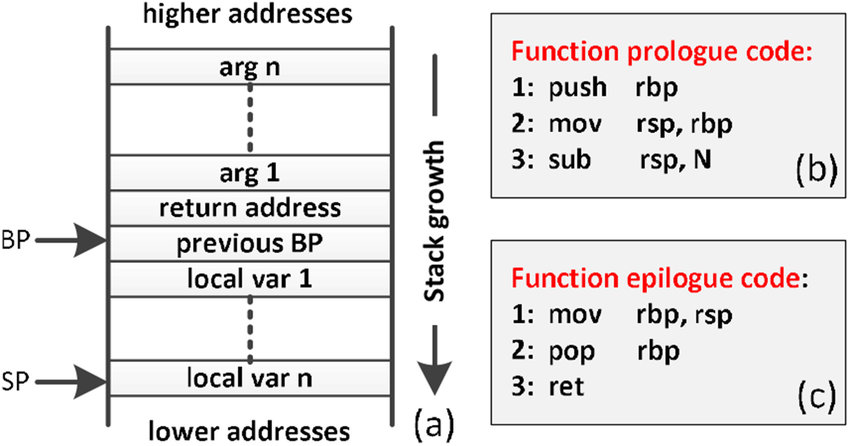
\includegraphics[width=0.8\textwidth]{day3/img/stack.jpg}
	\end{figure}
\end{frame}

\begin{frame}[fragile=singleslide,containsverbatim]{Quick Check: Memory Layout of C Program}
	Match the variables to the correct memory location:
	\begin{columns}
		\begin{column}{0.3\textwidth}
			\begin{figure}[H]
				\centering
				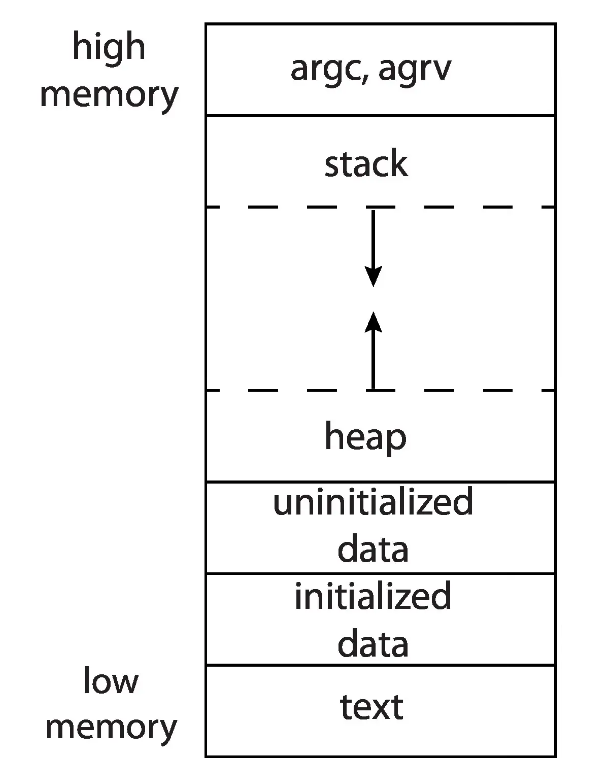
\includegraphics[width=\textwidth]{day3/img/mem-layout.png}
			\end{figure}
		\end{column}
		\begin{column}{0.7\textwidth}
			\begin{minted}[fontsize=\scriptsize,escapeinside=||]{c}
#include <stdio.h>
#include <stdlib.h>
int x;
int y = 15;
int main(int argc, char *argv[]) {
    int *values;
    int i;
    values = (int *)malloc(sizeof(int) * 5);
    for (i = 0; i < 5; i++)
        values[i] = i;
    return 0;
}
        \end{minted}
		\end{column}
	\end{columns}
\end{frame}

\begin{frame}[fragile=singleslide,containsverbatim]{Quick Check: Memory Layout of C Program (Answer)}
	\begin{figure}[H]
		\centering
		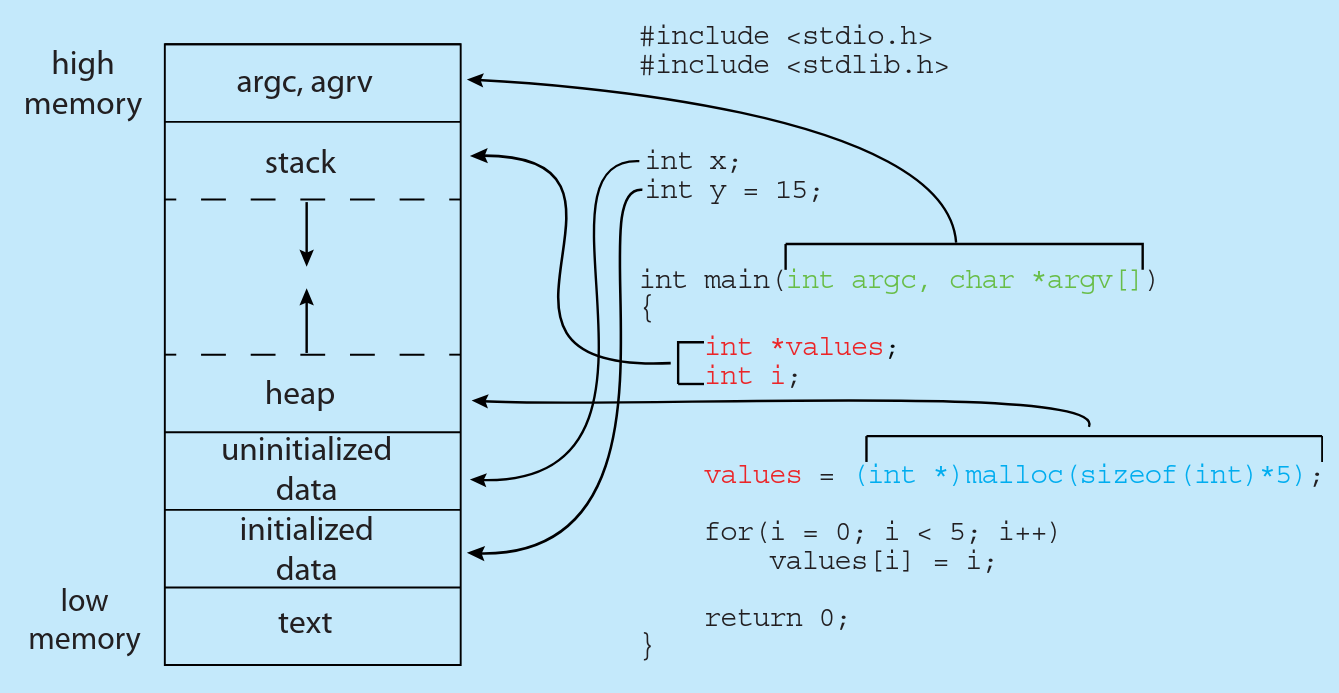
\includegraphics[width=0.9\textwidth]{day3/img/answer-layout.png}
	\end{figure}
\end{frame}

\subsection{Process Schedule}

\begin{frame}[fragile]{Process Schedule}
	\begin{itemize}
		\item \textbf{Non-preemptive}: The process must finish its execution before the OS can schedule another process.
		\item<2-> \textbf{Preemptive}: The OS can interrupt a process to schedule another one.
		      \begin{itemize}
			      \item<3-> Round Robin
			      \item<3-> Priority-based
		      \end{itemize}
	\end{itemize}
	\onslide<3->{
		\begin{figure}[H]
			\centering
			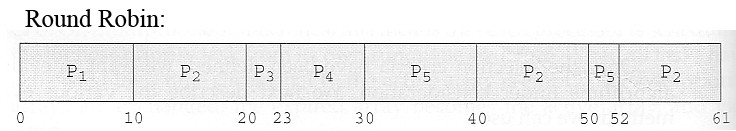
\includegraphics[width=0.6\textwidth]{day3/img/gantt.jpg}
		\end{figure}
		\begin{itemize}
			\item<4-> \emoji{star} \textbf{Also decide which process to run on which core.} (Control by \textbf{Core Affinity})
		\end{itemize}
	}
\end{frame}

\begin{frame}[fragile]{Process Switch}

	% Context Switch between two kernel processes:
	% \begin{figure}[ht!]
	%     \center
	%     \begin{tikzpicture}[x=0.8pt,y=0.8pt,yscale=-1,xscale=1]
	%     %uncomment if require: \path (0,300); %set diagram left start at 0, and has height of 300

	%     %Shape: Rectangle [id:dp0022237957984407863]
	%     \draw  [color={rgb, 255:red, 119; green, 187; blue, 221 }  ,draw opacity=1 ][fill={rgb, 255:red, 119; green, 187; blue, 221 }  ,fill opacity=0.05 ] (6,58.43) -- (438,58.43) -- (438,234.29) -- (6,234.29) -- cycle ;
	%     %Straight Lines [id:da4498626232311549]
	%     \draw [color={rgb, 255:red, 255; green, 136; blue, 153 }  ,draw opacity=1 ]   (38,123.43) -- (135,123.43) ;
	%     \draw [shift={(138,123.43)}, rotate = 180] [fill={rgb, 255:red, 255; green, 136; blue, 153 }  ,fill opacity=1 ][line width=0.08]  [draw opacity=0] (8.93,-4.29) -- (0,0) -- (8.93,4.29) -- cycle    ;
	%     %Straight Lines [id:da4226129673115242]
	%     \draw [color={rgb, 255:red, 255; green, 136; blue, 153 }  ,draw opacity=1 ]   (151.71,109.71) -- (140.12,121.31) ;
	%     \draw [shift={(138,123.43)}, rotate = 315] [fill={rgb, 255:red, 255; green, 136; blue, 153 }  ,fill opacity=1 ][line width=0.08]  [draw opacity=0] (8.93,-4.29) -- (0,0) -- (8.93,4.29) -- cycle    ;
	%     %Straight Lines [id:da24204008474623473]
	%     \draw [color={rgb, 255:red, 255; green, 136; blue, 153 }  ,draw opacity=1 ]   (138,123.43) -- (138,165) ;
	%     %Straight Lines [id:da12426250382299653]
	%     \draw [color={rgb, 255:red, 255; green, 136; blue, 153 }  ,draw opacity=1 ]   (138,165) -- (237.71,165) ;
	%     \draw [shift={(240.71,165)}, rotate = 180] [fill={rgb, 255:red, 255; green, 136; blue, 153 }  ,fill opacity=1 ][line width=0.08]  [draw opacity=0] (8.93,-4.29) -- (0,0) -- (8.93,4.29) -- cycle    ;
	%     %Straight Lines [id:da40164286447171516]
	%     \draw [color={rgb, 255:red, 119; green, 187; blue, 221 }  ,draw opacity=1 ]   (240.71,152.71) -- (240.71,177.29) ;
	%     %Straight Lines [id:da38281948784259523]
	%     \draw [color={rgb, 255:red, 119; green, 119; blue, 170 }  ,draw opacity=1 ]   (240.71,165.43) -- (316,165.43) ;
	%     %Straight Lines [id:da8211978963630775]
	%     \draw [color={rgb, 255:red, 119; green, 119; blue, 170 }  ,draw opacity=1 ]   (316,165.43) -- (316,144.43) ;
	%     \draw [shift={(316,141.43)}, rotate = 90] [fill={rgb, 255:red, 119; green, 119; blue, 170 }  ,fill opacity=1 ][line width=0.08]  [draw opacity=0] (8.93,-4.29) -- (0,0) -- (8.93,4.29) -- cycle    ;
	%     %Straight Lines [id:da9723145334004362]
	%     \draw [color={rgb, 255:red, 119; green, 119; blue, 170 }  ,draw opacity=1 ]   (316,141.43) -- (335,141.43) -- (418,141.43) ;
	%     \draw [shift={(421,141.43)}, rotate = 180] [fill={rgb, 255:red, 119; green, 119; blue, 170 }  ,fill opacity=1 ][line width=0.08]  [draw opacity=0] (8.93,-4.29) -- (0,0) -- (8.93,4.29) -- cycle    ;
	%     %Straight Lines [id:da6787843944387311]
	%     \draw [color={rgb, 255:red, 255; green, 136; blue, 153 }  ,draw opacity=1 ]   (209,180.86) -- (224.72,167.38) ;
	%     \draw [shift={(227,165.43)}, rotate = 139.4] [fill={rgb, 255:red, 255; green, 136; blue, 153 }  ,fill opacity=1 ][line width=0.08]  [draw opacity=0] (8.93,-4.29) -- (0,0) -- (8.93,4.29) -- cycle    ;
	%     %Straight Lines [id:da580092866214728]
	%     \draw [color={rgb, 255:red, 119; green, 119; blue, 170 }  ,draw opacity=1 ]   (298.71,124.14) -- (313.88,139.31) ;
	%     \draw [shift={(316,141.43)}, rotate = 225] [fill={rgb, 255:red, 119; green, 119; blue, 170 }  ,fill opacity=1 ][line width=0.08]  [draw opacity=0] (8.93,-4.29) -- (0,0) -- (8.93,4.29) -- cycle    ;

	%     % Text Node
	%     \draw (23,70.29) node [anchor=north west][inner sep=0.75pt]  [font=\normalsize,color={rgb, 255:red, 119; green, 187; blue, 221 }  ,opacity=1 ] [align=left] {Kernel Space};
	%     % Text Node
	%     \draw (47,107) node [anchor=north west][inner sep=0.75pt]  [font=\small] [align=left] {Kernel thread};
	%     % Text Node
	%     \draw (327,105) node [anchor=north west][inner sep=0.75pt]  [font=\small] [align=left] {Another\\Kernel thread};
	%     % Text Node
	%     \draw (153,98) node [anchor=north west][inner sep=0.75pt]  [font=\small,color={rgb, 255:red, 255; green, 136; blue, 153 }  ,opacity=1 ] [align=left] {Trap (timer)};
	%     % Text Node
	%     \draw (209,183.86) node [anchor=north] [inner sep=0.75pt]  [font=\small,color={rgb, 255:red, 255; green, 136; blue, 153 }  ,opacity=1 ] [align=left] {call switch\_to};
	%     % Text Node
	%     \draw (59,123) node [anchor=north west][inner sep=0.75pt]  [color={rgb, 255:red, 255; green, 136; blue, 153 }  ,opacity=1 ] [align=left] {dummy};
	%     % Text Node
	%     \draw (342,140.43) node [anchor=north west][inner sep=0.75pt]  [color={rgb, 255:red, 119; green, 119; blue, 170 }  ,opacity=1 ] [align=left] {dummy};
	%     % Text Node
	%     \draw (231,135) node [anchor=north west][inner sep=0.75pt]  [color={rgb, 255:red, 119; green, 187; blue, 221 }  ,opacity=1 ] [align=left] {ret};
	%     % Text Node
	%     \draw (128,167) node [anchor=north] [inner sep=0.75pt]  [font=\small,color={rgb, 255:red, 255; green, 136; blue, 153 }  ,opacity=1 ] [align=left] {P0 Trap Handler};
	%     % Text Node
	%     \draw (333,168) node [anchor=north] [inner sep=0.75pt]  [font=\small,color={rgb, 255:red, 255; green, 136; blue, 153 }  ,opacity=1 ] [align=left] {\textcolor[rgb]{0.47,0.47,0.67}{P1 Trap Handler}};
	%     % Text Node
	%     \draw (245,108) node [anchor=north west][inner sep=0.75pt]  [font=\small,color={rgb, 255:red, 119; green, 119; blue, 170 }  ,opacity=1 ] [align=left] {Trap exit};
	%     \end{tikzpicture}
	% \end{figure}
	\begin{figure}[H]
		\centering
		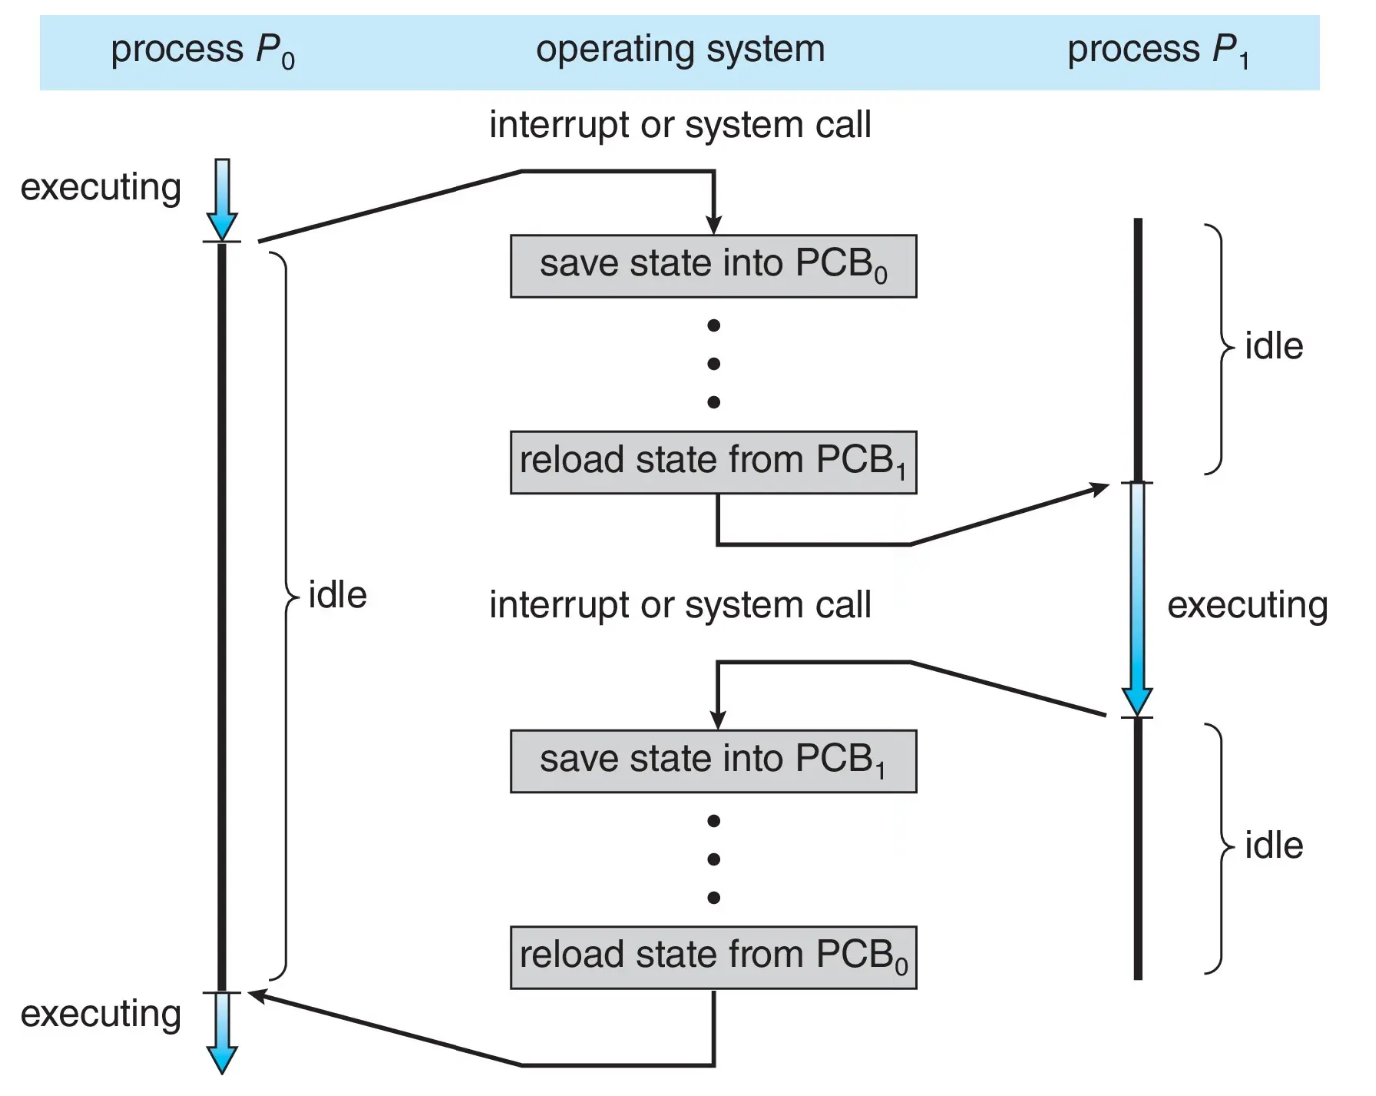
\includegraphics[width=0.6\textwidth]{day3/img/switch1.png}
	\end{figure}
\end{frame}


\subsection{Inter-Process Communication (IPC)}

\begin{frame}[fragile]{Inter-Process Communication}
	\only<1>{
		\textbf{Why?}
		\begin{itemize}
			\item Processes within a host may be \textbf{cooperating}
		\end{itemize}
		\begin{figure}[H]
			\centering
			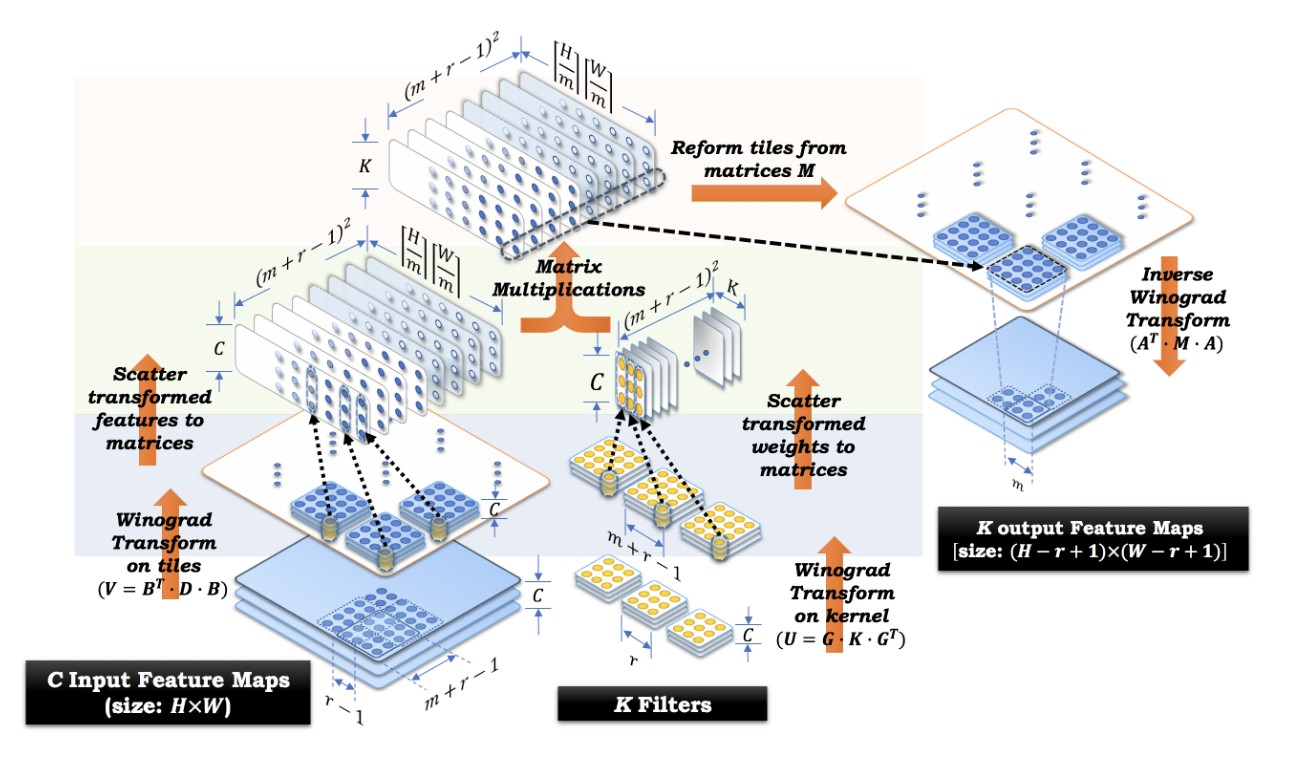
\includegraphics[width=0.65\textwidth]{day3/img/winograd.jpg}
		\end{figure}
	}

	\only<2>{
		\textbf{How?}
		\begin{itemize}
			\item \textbf{Message Passing}: We use \textbf{MPI} to send / receive messages.
			\item Shared Memory, Signal, Pipe, Socket...
		\end{itemize}
		\begin{figure}[H]
			\centering
			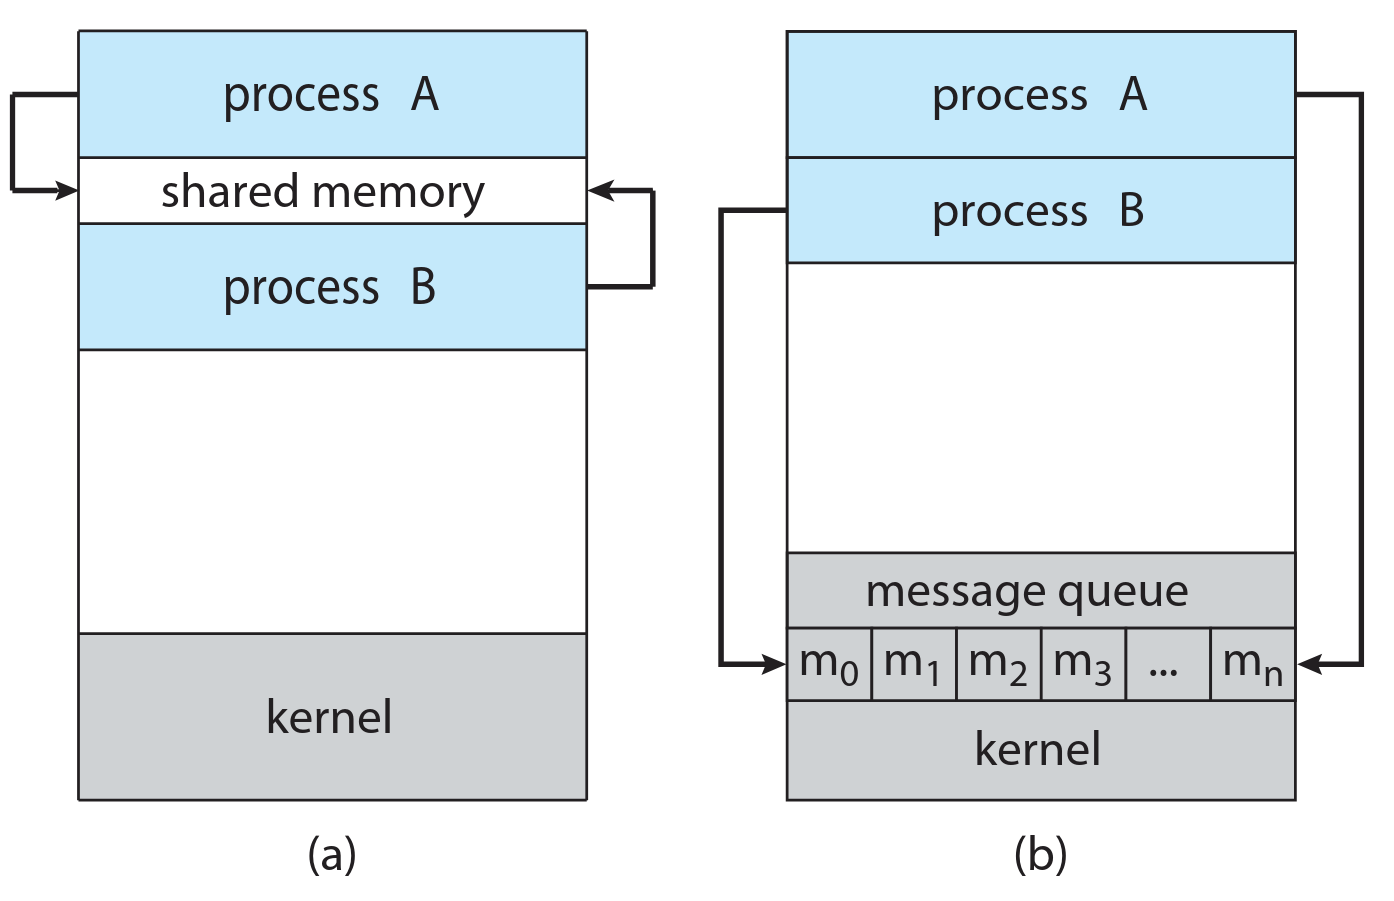
\includegraphics[width=0.5\textwidth]{day3/img/ipc.png}
		\end{figure}
	}
\end{frame}

\begin{frame}[fragile]{Inter-Process Communication}
	Disadvantages of IPC: \textbf{It's too heavy!} \emoji{woozy-face}
	\begin{itemize}
		\item Due to \textbf{isolation}, processes do not share address space.
		\item<2-> For message passing:
		      \begin{itemize}
			      \item Need to maintain a \textbf{message queue} for each process.
			      \item Data need to be \textbf{copied between address spaces}.
		      \end{itemize}
		\item<3-> For shared memory:
		      \begin{itemize}
			      \item Synchronization is needed
			      \item It's \textbf{complex for OS to manage}.
		      \end{itemize}
		\item<4-> Must flush cache when switching between processes. (Why?)
	\end{itemize}
	\onslide<5>{ \emoji{thinking} Is there a better way? }
\end{frame}

\section{Thread}

\begin{frame}[fragile]{Thread: Light-Weight Process}
	\only<2>{
		\begin{figure}[H]
			\centering
			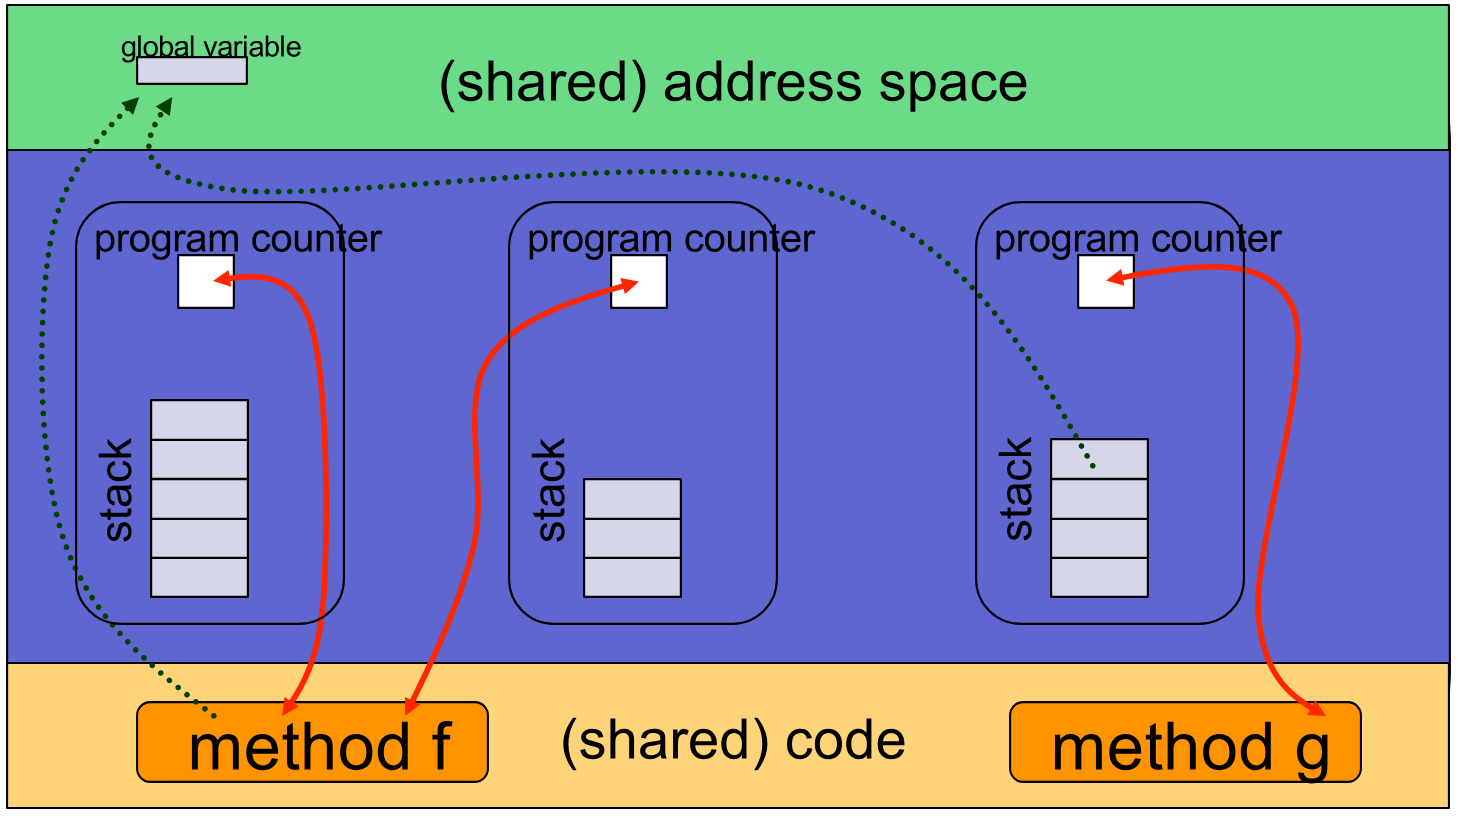
\includegraphics[width=0.8\textwidth]{day3/img/thread.png}
		\end{figure}
	}
	\only<1>{
		\begin{itemize}
			\item \emoji{star} A thread is a \textbf{basic unit of execution} within a process. Each thread has its own:
			      \begin{itemize}
				      \item Thread ID
				      \item Program counter
				      \item Register set
				      \item Stack
			      \end{itemize}
			\item Shares the following with other threads within the same process:
			      \begin{itemize}
				      \item Code section
				      \item Data section
				      \item The heap (dynamically allocated memory)
				      \item Open files and signals
			      \end{itemize}
			\item \textbf{Concurrency}: A multi-threaded process \textbf{can do multiple things at once}
		\end{itemize}
	}
\end{frame}

% \begin{frame}[fragile]{OpenMP: Multi-Thread in Practice}
% OpenMP
% \end{frame}

\section{Virtual Memory}

\begin{frame}[fragile]{Virtual Memory}
	\emoji{bullseye} Why do we need virtual memory?
	\begin{itemize}
		\item Virtual memory is another abstraction layer between process and physical memory.
		      \begin{itemize}
			      \item<1-> \textbf{Isolation}: Each process has its own address space.
			      \item<2-> \textbf{Protection}: Deny the process from accessing other processes' or privileged memory.
			      \item<3-> \textbf{Efficiency}: Support Copy-on-Write, can run a partially loaded program.
		      \end{itemize}
	\end{itemize}

	\onslide<4->{
		\emoji{thinking} How to implement virtual memory?
		\begin{itemize}
			\item We'll only talk about \textbf{Paging} today.
		\end{itemize}
	}

\end{frame}

\begin{frame}[fragile]{Paging in a Nutshell}

	\begin{itemize}
		\item<1-> \textbf{Page and Frame}
		      \begin{itemize}
			      \item Physical memory is split into \textbf{fixed-size frames}.
			      \item Virtual memory is split into \textbf{fixed-size pages}.
		      \end{itemize}
		\item<2-> \textbf{Memory Mapping}
		      \begin{itemize}
			      \item Hardware support: \textbf{MMU} (Memory Management Unit)
			      \item Function: Translate \textbf{virtual page} to \textbf{physical frame}
			      \item Data structure: \textbf{Page Table}
		      \end{itemize}
		\item<3-> \textbf{Page Fault}
		      \begin{itemize}
			      \item If a page is not in physical memory, a page fault occurs.
			      \item The OS will load the page from disk to physical memory, and update the page table.
		      \end{itemize}
	\end{itemize}

\end{frame}

\begin{frame}[fragile]{Paging in practice}

	\begin{columns}
		\begin{column}{0.3\textwidth}
			\begin{figure}[H]
				\centering
				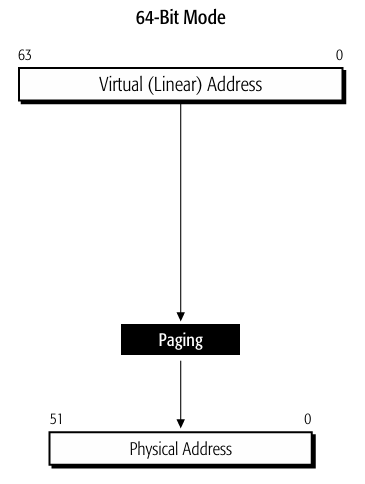
\includegraphics[width=\textwidth]{day3/img/page.png}
			\end{figure}
		\end{column}
		% \onslide<2->{
		\begin{column}{0.7\textwidth}
			\begin{figure}[H]
				\centering
				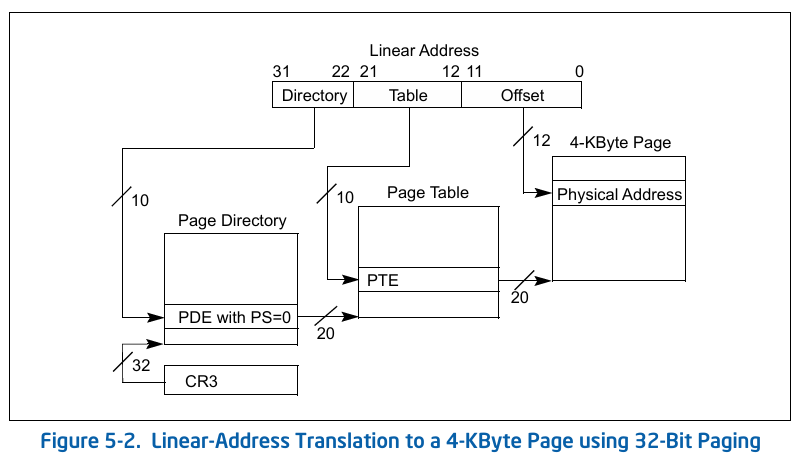
\includegraphics[width=\textwidth]{day3/img/page-table.png}
			\end{figure}
		\end{column}
		% }
	\end{columns}

\end{frame}


\begin{frame}[fragile]{Takeaways}
	\emoji{star} Important concepts that you should remember today:
	\begin{itemize}
		\item Operating System:\textbf{a resource abstractor and resource allocator.}
		\item Process: \textbf{a unit of resource allocation and protection.}
		\item Thread: \textbf{basic unit of execution} within a process.
		\item Others: Memory Hierarchy, Stack Frame, etc.
	\end{itemize}
\end{frame}

% Q&A
\begin{frame}[standout]
	\Huge\textsc{Thank You}

	\vfill

	\LARGE\textsc{Any Questions?}
\end{frame}

\end{document}
